\chapter{Projektmanagement}

Das folgende Kapitel beschäftigt sich mit der Führung und Kontrolle des Projekts. Das Projektmanagement, wie auch die spätere Entwicklung funktionieren agil. Um möglichst effizient auf Änderungen reagieren zu können, werden entsprechende Hilfsmittel verwendet.
%Im folgenden Kapitel werden Führung und Kontrolle des Projekts aufgezeigt. Das Projektmanagement funktioniert agil, dafür werden geeignete Hilfsmittel eingesetzt. 

\section{Ausgangslage}
Aus dem Forschungsprojekt \gls{Intuitive Knowledge Connectivity}\footnote{\url{https://www.hslu.ch/en/lucerne-university-of-applied-sciences-and-arts/research/projects/detail/?pid=3334}} ging neben einer Publikation\footnote{\citep{ikcpaper:hslu}} auch ein Software-Prototyp\footnote{\url{http://demo.ikc.today/nodeDetail.html}} (\gls{ikc-core}) hervor. Das Projekt beschäftigt sich mit einem intuitiven Umgang mit Daten aus diversen Cloud-Dienstleistern, beispielsweise \gls{Dropbox}, \gls{Evernote} und vielen mehr. Diese werden, ebenfalls \gls{cloudbasiert}, gespeichert und verteilt. Der Mehrwert entsteht durch die Verknüpfung der verschiedenen Daten zu einem gesamtheitlichen Ganzen. Diese Verknüpfungen sind be\-nutzer\-bas\-iert und werden mithilfe einer Graph-Datenbank gehandhabt.

Da beide Projektmitarbeiter ebenfalls am Forschungsprojekt tätig sind, ist das Grundlagewissen bereits grösstenteils vorhanden. Die Arbeit am Forschungsprojekt und am \gls{PAWI} verlaufen parallel weiter. Um eine adäquate Trennung der beiden Projekte zu gewährleisten, wird im \autoref{sec:scope} näher auf die Gegebenheiten eingegangen.

\subsection{Internationale Projektorganisation}
\label{subsec:international}
Damit Andreas Waldis ein Team-Mitglied während des Projekts in den Vereinigten Staaten im Austauschsemester weilt, müssen einige zusätzliche organisatorische Massnahmen ergriffen werden. Diese umfassen die folgenden Tools und Arbeitsweisen:
\begin{itemize}
\item Die Zeitverschiebung zwischen Luzern (\textit{UTC+01:00}) und West Lafayette (\textit{UTC-05:00}) beträgt sechs Stunden. Daher werden Sitzungen überwiegend nachmittags nach 14:00 angesetzt. 
\item Projektplanung: Die Projektdauer wurde für diesen speziellen Fall um sechs Wochen auf Ende Januar erweitert. Dies ermöglicht die verschiedenen Teammitglieder entsprechend ihrer Auslastung zu arbeiten. Insbesondere für Andreas Waldis, welcher bereits im Dezember die Abschlussprüfungen hat. 
\end{itemize}

\subsection{Werkzeuge}

Es werden verschiedene Werkzeuge verwendet, um eine möglichst optimale Kommunikation und Kollaboration zu gewährleisten. Dazu gehören:
\begin{enumerate}
% \item \textbf{Slack}: Ein Messenger, welcher für die Verwendung im professionellen Umfeld ausgelegt ist. So können beispielsweise verschiedenet Cloud-Services integriert werden.\footnote{\url{https://slack.com/}}
\item \textbf{Skype}\footnote{\url{https://www.skype.com/de/}} \& \textbf{Discord}\footnote{\url{https://discordapp.com/}}: Beides Werkzeuge für Video- und Audio-Sitzungen. Skype ist wohlbekannt. Discord hingegegen ist spezialisiert für Gamer und beinhaltet ein umfangreicheres Chat-System.
\item \textbf{Targetprocess}\footnote{\url{https://www.targetprocess.com}}: Vergleichbar mit dem bekannten ScrumDo\footnote{\url{http://www.scrumdo.com}}. Im Gegensatz dazu verfügt Targetprocess jedoch über eine moderne Benutzeroberfläche und scheint für den vorliegenden Verwendungszweck allgemein geeigneter zu sein.
\item \textbf{Sharelatex}\footnote{\url{https://www.sharelatex.com}}: Online Kollaborationstool für Latex. Anstelle von lokalen Installationen in einem gemeinsamen Versions\-verwalt\-ungs\-sys\-tem, wird einfach direkt online am selben Dokument gearbeitet.
\item \textbf{draw.io}\footnote{\url{https://www.draw.io}}: Werkzeug, um online Diagramme zu zeichnen. Diese können ebenfalls gemeinsam und gleichzeitig gezeichnet werden. Zusätzlich ist es ideal, um schnell und einfach alles Mög\-liche zu zeichnen.
\end{enumerate}

\section{Scope}
\label{sec:scope}

Die Schwierigkeit liegt zu einem grossen Teil in der Abgrenzung zum parallellaufenden Projekt \gls{IKC}. Grundsätzlich gehört jegliche Arbeit im zweidimensionalen Bereich zum \gls{PAWI}. Der bestehende \gls{ikc-core} wird soweit vorbereitet, dass die Visualisierung ohne Zusatzaufwand integriert werden kann. Hierzu gehören Arbeiten betreffend Schnittstellen, Absenden von allfälligen \gls{Event}s und dergleichen. Das Ziel ist die Entwicklung eines Zusatzmoduls zum \gls{ikc-core}, welches mittels definierten Schnittstellen ein- und angebunden werden kann. Die genaue Spezifikation ist im Lösungskonzept noch zu erarbeiten.

Weiter ist zu betonen, dass die intuitive Bedienung (\gls{Usability} oder auch \gls{User Experience}) nach bestem Wissen und Gewissen angestrebt wird. Allerdings handelt es sich bei den Projektmitarbeitern um Informatiker ohne grundlegende Kenntnisse in den angesprochenen Bereichen. Die Benutzeroberfläche wird darum nach dem subjektiven Befinden des Projektpartners und den beiden Projektmitarbeitern entwickelt.

\section{Projektstrukturplan}
Die \autoref{fig:projektstrukturplan} gewährt einen Überblick über das Projekt. Sie stellt die wichtigsten Bereiche und Phasen dar, in welche die Arbeit grob eingegliedert werden kann:
\begin{enumerate}
    \item Die \textbf{Projektführung} beinhaltet die Planung des Vorhabens über den gegebenen Zeitraum. Ständige Kontrolle des Ist- gegenüber dem Soll-Zustand kann gegebenenfalls zur Steuerung oder Anpassungen des Zeitplans führen. Im Gegensatz zu den anderen Bereichen wird die Projektführung über die volle Projektdauer ausgeführt. Da das Projekt agil organisiert ist, liegt das Augenmerk auf der Priorisierung der Anforderungen.
    \item In der \textbf{Konzeption} werden neben den Anforderungen auch mög\-li\-che Lösungsansätze in den Bereichen Architektur, Schnittstellen und \gls{User Interface}/\gls{User Experience} gesammelt.
    \item Nach der Recherche von Lö\-sungs\-an\-sätz\-en muss allenfalls die Auswahl an Mög\-li\-chkei\-ten eingeschränkt werden. Eine anschliessende Testphase erleichtert die \textbf{Evaluation und Auswahl} der Lösungsvariante.
    \item Nun beginnt die Phase der eigentlichen \textbf{Entwicklung}. Auf Basis der bestehenden Tests wird die Visualisierung mit allen erforderlichen Komponenten erarbeitet. Der Schwerpunkt liegt auf der Gestik und dem \gls{Responsive Design}. Ein abschliessendes Testing des Systems stellt sicher, dass die Integration beginnen kann.
    \item Sobald die Visualisierung reibungslos funktioniert, wird sie in den bestehenden \gls{ikc-core} \textbf{integriert}. Alle Anforderungen werden erfüllt und anschliessend getestet.
    \item Nachdem die Entwicklungsarbeiten abgeschlossen sind, folgt der \textbf{Projektabschluss}. Dabei wird die endgültige Version des Projektreports erstellt und die Abschlusspräsentation gehalten.
\end{enumerate}

\newpage

\begin{landscape}
\begin{figure}[ht]
\centering
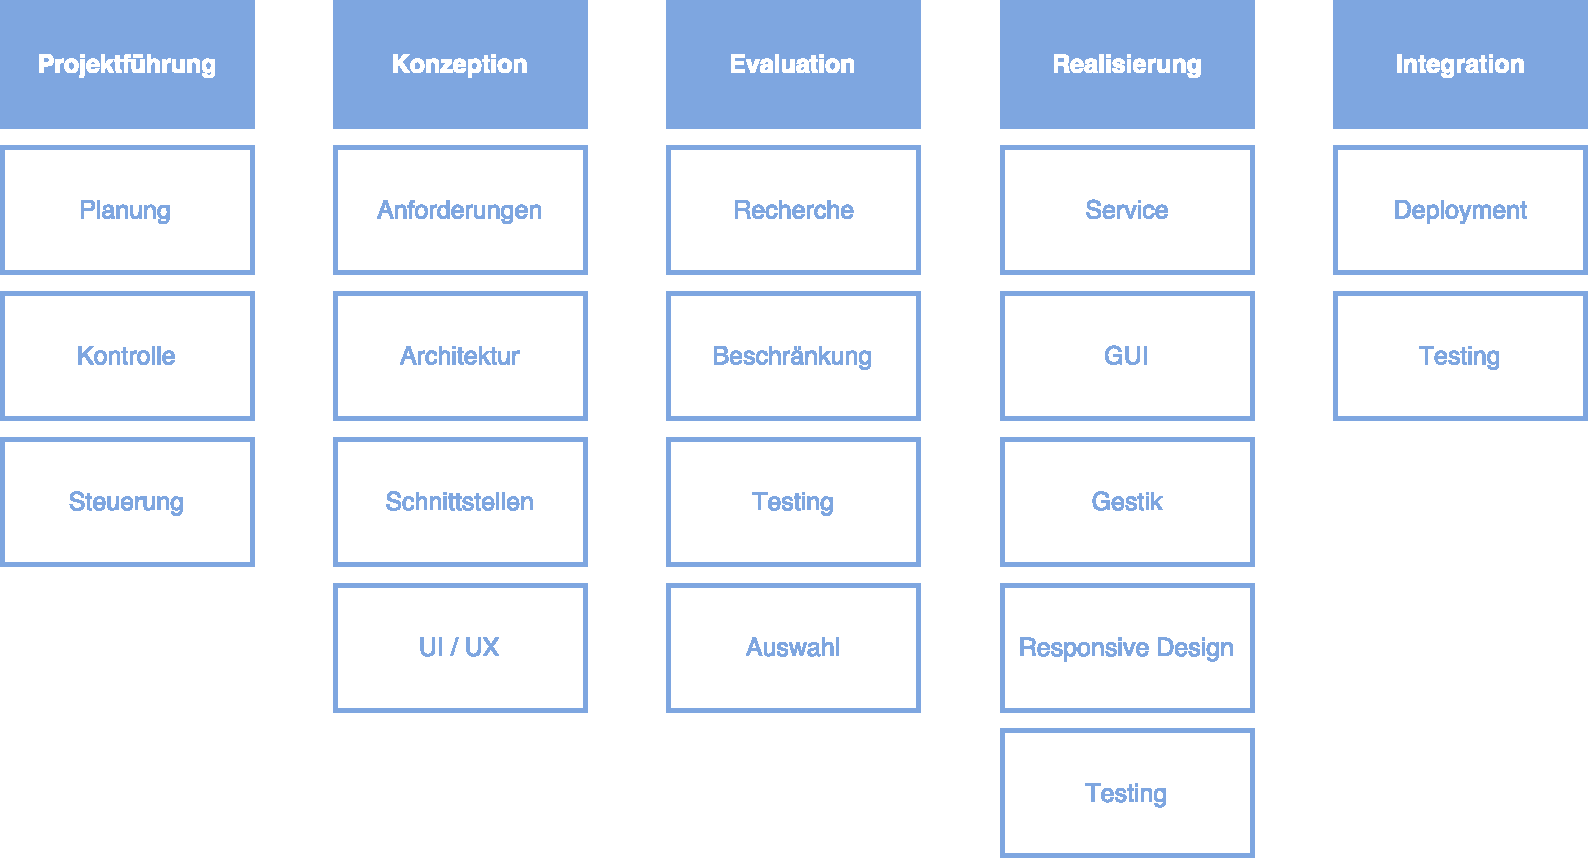
\includegraphics[width=1.5\textwidth]{Projektstrukturplan}
\caption{Projektstrukturplan}
\label{fig:projektstrukturplan}
\end{figure}
\end{landscape}

\newpage

\section{Rahmenplan}
Die Rahmenplanung, basierend auf dem Projektstrukturplan (\autoref{fig:rahmenplan}), repräsentiert die zeitliche Planung des Projekts. Dabei werden Kalenderwochen anstelle von Daten oder Schulwochen verwendet. Dies aufgrund des internationalen Rahmens, der damit verbundenen Zeitverschiebung und unterschiedlichen Stundenplänen. Enthalten sind alle Projektphasen, Sprints und Meilensteine, als auch alle Lieferobjekte welche im \autoref{lieferobjekte} weiter ausgeführt werden. Die Dauer der Sprints wird bewusst unterschiedlich ausgestaltet, um den verschiedenen Projektphasen und deren Inhalten Rechnung zu tragen.
%Die Sprints dauern absichtlich unterschiedlich lange, das deshalb, weil die Länge auf\-grund der verschiedenen Projektphasen und deren Inhalt zugeordnet worden ist. Weiter werden administrative Elemente durch blaue Färbung und Entwicklungs-Elemente durch rote Färbung gekennzeichnet.

Eine grosse Rolle in der Rahmenplanung spielen die Meilensteine. Sie unterteilen das Projekt in Phasen, welche dadurch klar voneinander getrennt sind. Ebenfalls sind sie eine wichtige Orientierungshilfe im Projekt und weisen den Weg damit das Projekt erfolgreich abgeschlossen werden kann. Die \autoref{tab:meilensteine} listet die Meilensteine auf.


\begin{longtable}{|p{1cm}|p{2cm}|p{8.5cm}|}
  \hline
    ID & Datum &  Beschreibung \\\hline
    M1 & 19.09.2016 & Administrativer Meilenstein: Kickoff\\\hline
    M2 & 09.10.2016 & Administrativer Meilenstein: Projektplanung abgeschlossen\\\hline
    M3 & 16.10.2016 & Entwicklung Meilenstein: Schnittstellen definiert\\\hline
    M4 & 06.11.2016 & Entwicklung Meilenstein: Evaluation Entscheid\\\hline
    M5 & 25.12.2016 & Entwicklung Meilenstein: Funktionsfähige Oberfläche umgesetzt\\\hline
    M6 & 15.01.2017 & Entwicklung Meilenstein: Integration in \gls{ikc-core} abgeschlossen\\\hline
    M7 & 22.01.2017 & Administrativer Meilenstein: 95\% erreicht\\\hline
    M8 & 30.01.2017 & Administrativer Meilenstein: PAWI Bericht Abgabe\\\hline
    M9 & 31.01.2017 & Administrativer Meilenstein: Präsentation\\\hline
    \caption{Meilensteine}
  \label{tab:meilensteine}
\end{longtable}

\newpage

\begin{landscape}
\begin{figure}[ht]
\centering
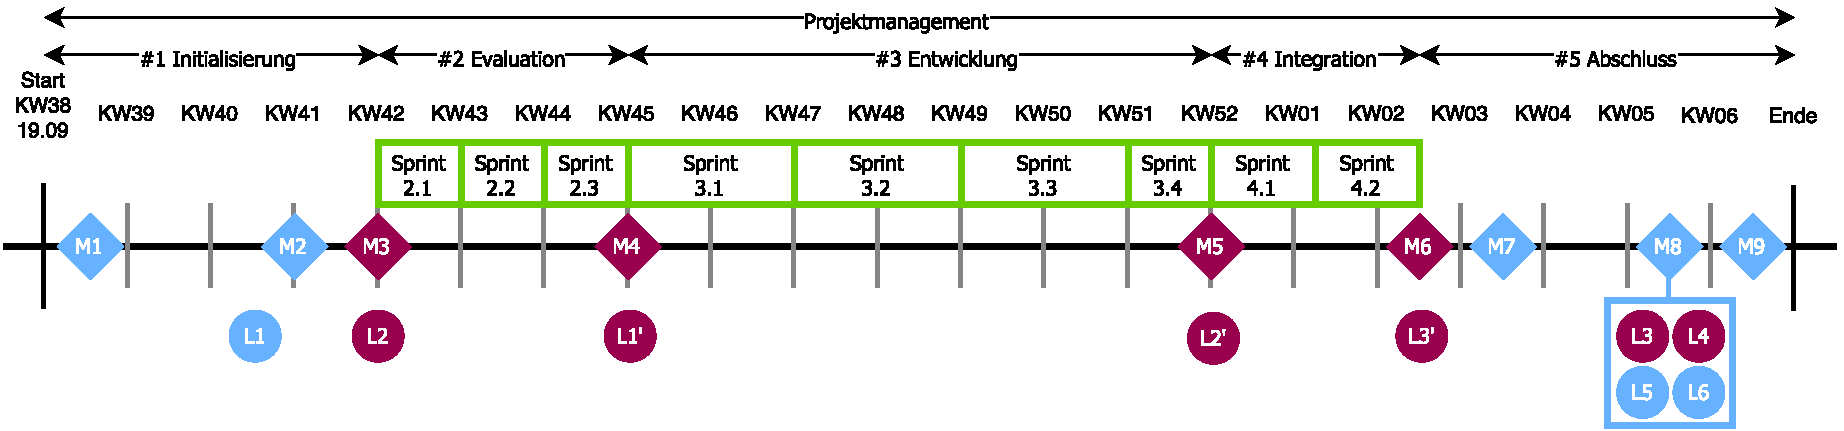
\includegraphics[width=1.7\textwidth]{Rahmenplan}
\caption{Rahmenplan}
\label{fig:rahmenplan}
\end{figure}
\end{landscape}

\newpage

\section{Projektziele} \label{projektziele}
Projektziele werden definiert, um den Erfolg an einigen ausgewählten Punkten zu überprüfen und sicherstellen zu können. Sie wurden in Absprache mit dem Kunden definiert. Die Ziele sind in der folgenden \autoref{tab:projekt-ziele} aufgelistet.

\begin{longtable}{|p{1cm}  | p{10.5cm}|}
  \hline
    ID &  Beschreibung \\\hline
    Z1 & Ergänzung zur bestehenden Benutzeroberfläche.\\\hline
    Z2 & Entwicklung nach dem Konzept \gls{mobile first}.\\\hline
    Z3 & Intuitive, visuelle und effiziente Interaktion mit einem \gls{Netzwerk}.\\\hline
    Z4 & Übersichtliche Visualisierung der \gls{Node}[s] und \gls{Link}[s].\\\hline
    Z5 & Erweiterung der Funktionalität mittels Sichten (\gls{View}s).\\\hline
    \caption{Projektziele}
  \label{tab:projekt-ziele}
\end{longtable}

\section{Anforderungen} \label{anforderungen}

Für die weitere Unterteilung in Arbeitspakete und \textit{Stories} werden die Anforderungen zunächst in Prosa gesammelt. Diese entstammen dem Kundenworkshop und der Aufgabenstellung, sind im Sinn der Projektziele (\autoref{projektziele}). Die Anforderungen werden unterschieden in funktionale und nicht-funktionale Anforderungen. Die funktionalen Anforderungen definieren direkt die Eigenschaften, (\autoref{tab:funktionale-anforderungen}). Im Gegensatz dazu definieren nicht-funktionale Anforderungen die Leistung und die Randbedingungen, aufgelistet in \autoref{tab:nicht-funktionale-anforderungen}.

Die Priorisierung erfolgt nach dem \gls{MoSCoW-System}:

\begin{longtable}{|p{1.5cm} | p{2.5cm} | p{7.2cm}|}
  \hline
    \# & Priorität & Beschreibung \\\hline
    M & Must Have & Bei dieser Anforderung handelt es sich um ein Muss, höchste Priorität.\\\hline
    S & Should Have & Diese Anforderung wird erwartet, normale Priorität.\\\hline
    C & Could Have & Tiefste Priorität, desiderata.\\\hline
    \caption{MosCow-Priorisierung}
  \label{tab:moscow}
\end{longtable}


\begin{longtable}{|p{1.5cm} | p{1.5cm} | p{8.1cm}|}
  \hline
    ID & Priorität & Beschreibung \\\hline
    A1.1 & M & Die zugrundeliegende Datenbasis kann mittels eines \gls{Netzwerk}[s] visualisiert werden. Jenes besteht aus Knoten und Kanten, welche gerichtet und beschriftet sind.\\\hline
    A1.2 & M & Die zu erarbeitende Visualisierung kann bidirektional mit dem \gls{ikc-core} interagieren. Änderungen am \gls{ikc-core} sind in der Visualisierung sichtbar. Es ist jedoch auch möglich Änderungen direkt in der Visualisierung vorzunehmen.\\\hline
    A1.3 & S & Mittels der Visualisierung können die grundlegenden Datenbankoperationen \textit{CREATE}, \textit{READ}, \textit{UPDATE} und \textit{DELETE} (CRUD) teilweise direkt auf der Datenbasis des \gls{ikc-core}[s] angewendet werden.\\\hline
    A1.3.1 & S & Es können sowohl Knoten aus der Visualisierung als auch aus der Datenbasis\footnote{Hier ist die Datenbasis des \gls{ikc-core}[s] gemeint.} gelöscht werden. Diese Vorgänge können klar unterschieden werden.\\\hline
    A1.3.2 & M & Knoten ohne Kanten können in der Visualisierung abgebildet werden.\\\hline
    A1.3.3 & M & Knoten können in der Visualisierung erstellt werden.\\\hline
    A1.4 & M & Der Prototyp kann auf Smartphones und Tablets benutzt werden.\\\hline
    A1.5 & S & Der Prototyp kann auf Laptops und Desktop-Computern benutzt werden.\\\hline    
    A1.6 & M & Mit Hilfe verschiedener Kriterien (beispielsweise Kontext oder Nachbarschaft) kann ein Teil eines \gls{Netzwerk}[s] visualisiert werden.\footnote{Die Visualisierung eines Teils eines \gls{Netzwerk}[s]  wird später als \gls{View} bezeichnet.}\\\hline 
    A1.6.1 & S & Diese Visualisierungen (ein Teil des \gls{Netzwerk}[s]) können unabhängig von der Datenbasis persistiert werden. Es können, zusätzlich zu den Knoten und Kanten, auch deren relative Positionen in der Visualisierung gespeichert werden.\\\hline 
    A1.7 & C & Der Prototyp kann (unter anderem) mit \gls{Drag'n'Drop} bedient werden.\\\hline
    A1.7.1 & S & Bidirektionale und unbeschriftete Verknüpfungen zwischen visualisierten Knoten können erstellt werden.\\\hline
    A1.7.2 & M & Ein, in der bestehenden Benutzeroberfläche\footnote{\gls{ikc-core}}, mittels der Suche gefundener Knoten kann direkt in die Visualisierung übernommen werden.\\\hline 
    A1.7.3 & S & Ein mittels der Suchfunktion gefundener Knoten kann auf einen bestehenden Knoten gezogen werden, um mit diesem eine Kante zu bilden.\\\hline 
    A1.7.4 & S & Knoten können innerhalb des Diagramms frei positioniert werden.\\\hline 
    A1.8 & M & Die Visualisierung kann innerhalb der bestehenden \gls{ikc-core} Oberfläche genutzt werden.\\\hline 
    A1.9 & S & In der Visualisierung könnnen auch Knoten mit mehr als sieben Kindknoten dargestellt werden: Sind mehr als sieben Kindknoten vorhanden, wird anstelle einer Repräsentation jedes einzelnen Knotens auf eine Liste gewechselt. Diese Liste kann zusätzlich mit einer Such- und oder Filterfunktion versehen werden.\\\hline  
    A1.10 & C & Die von einem Knoten aus- und eingehenden Kanten können auf- und zugeklappt (sichtbar-unsichtbar) werden.\\\hline
    A1.10.1 & C & Einzelne Kanten können individuell zugeklappt/ausgeblendet werden.\\\hline
     
    \caption{Funktionale Anforderungen}
  \label{tab:funktionale-anforderungen}
\end{longtable}

\begin{longtable}{|p{1.5cm} | p{1.5cm} | p{8.1cm}|}
  \hline
    ID & Priorität & Beschreibung \\\hline
    A2.1 & M & Bestehende Komponenten des \gls{ikc-core}[s] werden, wo möglich, wiederverwendet bzw. erweitert (nachhaltige Entwicklung).\\\hline
    A2.2 & M & Die Visualisierung kann in verschiedenen Projekten wiederverwendet werden.\\\hline
    A2.3 & M & Die Visualisierung wird im \gls{ikc-core} integriert (Deployment).\\\hline
    A2.4 & M & Die Visualisierung wird parallel zum \gls{ikc-core} weiterentwickelt. Die Basis für die Visualisierung bildet ein Klon der bestehenden Codebasis aus dem Versionkontrollsystem. Ist die Entwicklung abgeschlossen, werden die beiden Entwicklungsstände mittels eines neuen Astes (Branch) zusammengeführt.\\\hline
    A2.5 & M & Jegliche Daten werden auf der Dropbox des Benutzers persistiert.\\\hline
    A2.6 & S & Es wird eine intuitive, effiziente Bedienung angestrebt. Ein Mass für die Effizienz: $\frac{\text{Taps}}{\text{Task}}$\\\hline
    A2.7 & M & Randbedingungen 180h pro Person\\\hline
    A2.8 & S & Die Arbeit können in einem Arbeitsjournal, mindestens mit Angaben von Datum, Anzahl Stunden, Arbeitsschritt/Thema, nachverfolgt werden.\\\hline
    \caption{Nicht funktionale Anforderungen}
  \label{tab:nicht-funktionale-anforderungen}
\end{longtable}

\section{Risikoanalyse}\label{risikoanalyse}

In folgender \autoref{tab:risikoanalyse} werden mögliche Risiken behandelt. Die Wahrscheinlichkeit ist mit P abgekürzt. R steht für Risiko und S für den Schaden, welcher mittels $P*R=S$ berechnet wird.

\clearpage

\begin{longtable}{|p{0.5cm} | p{7cm} | p{1cm}|  p{1cm}|  p{1cm}|}
  \hline
    ID & Beschreibung &  P & R & S \\\hline
    R1 & Wie in \autoref{subsec:international} bereits angesprochen wird das Projekt in einem \textbf{internationalen Rahmen} durchgeführt. Dies birgt einige Herausforderungen und bringt auch Riksiken mit sich: Die grösste Schwierigkeit bildet sicherlich die Zeitverschiebung. Aber auch die geographische Distanz und die lediglich im digitalen Rahmen gehaltenen Sitzungen sind nicht zu unterschätzen.\newline
    Um dieser Problematik zu entgegnen, werden diverse Kommunikationswege, vorwiegend verschiedenen On\-line-Platt\-for\-men, benutzt. Diese sollen trotz den Gegebenheiten die Kollaboration und den Austausch unterstützen und fördern. & 1 & 3 & 3\\\hline
    R2 & Die Abgrenzung vom laufenden Projekt \textbf{\acrshort{IKC}} (vgl. \autoref{sec:scope}) ist klar festzulegen und einzuhalten. So können Überschneidungen und Unklarheiten verhindert werden.\newline
    Vollständige und detaillierte Arbeitsjournale, wie auch Protokolle bieten dabei eine wichtige Hilfestellung.  & 2 & 1 & 2\\\hline
    R3 & Die Zahl der Anforderungen ist hoch. Im Rahmen der \textbf{360 zu leistenden Stunden} ist es wichtig, sich nicht in Details oder in der Ausarbeitung jeglicher Finessen zu verlieren.\newline
    Darum ist es umso wichtiger, die Anforderungen klar zu priorisieren und auch entsprechend abzuarbeiten.  & 3 & 1 & 3\\\hline
    \caption{Risikoanalyse}
  \label{tab:risikoanalyse}
\end{longtable}

\section{Lieferobjekte}\label{lieferobjekte}

Neben den in der Aufgabenstellung vorgegebenen Lieferobjekte (\autoref{tab:set-lieferobjekte}) sind noch zusätzliche, interne Lieferobjekte (\autoref{tab:add-lieferobjekte}) festlegt. Diese sind lediglich als Unterstützung der Projektkontrolle, eine Art Orientierungshilfe, gedacht.

\begin{longtable}{|p{1cm} | p{2cm} | p{8.1cm}|}
  \hline
    ID & Datum &  Beschreibung \\\hline
    L1 & 30.09.2016 & Projektplanung.\\\hline
    L2 & 07.10.2016 & Anforderungskatalog.\\\hline
    L3 & 17.10.2016 & Lösungskonzept inkl. Schnittstellendefinition.\\\hline
    L4 & 30.01.2017 & Funktionsfähige Software mit folgenden Eigenschaften:
    \begin{itemize}
        \item Integriert bestehender Prototyp auf Basis \hyperref[react]{\textit{React}} mit allen \textbf{\textit{CRUD}}\footnote{Create Read Update Delete} Funktionen und Schnittstellen zu \gls{Dropbox} und \gls{Evernote}.
        \item Möglichkeit zur visuellen Interaktion mit einem 
            Teil eines \gls{Netzwerk}[s]: Knoten können per \gls{Drag'n'Drop} verknüpft werden
        \item Die Applikation läuft auf dem Mobile, Tablet, Laptop und Desktop (in Priorität der Reihenfolge) $\rightarrow$ responsive CSS Template\footnote{\gls{Responsive Design}} verwenden.
    \end{itemize}
    \\\hline
    L5 & 30.01.2017 & Dokumentierter Sourcecode (für Methoden und Parameter).\\\hline
    L6 & 30.01.2017 & Benutzerhandbuch.\\\hline
    L7 & 30.01.2017 & \gls{PAWI}-Bericht.\\\hline
    \caption{Vorgegebene Lieferobjekte}
  \label{tab:set-lieferobjekte}
\end{longtable}
 
\begin{longtable}{|p{1cm} | p{2cm} | p{8.1cm}|}
  \hline
    ID & Datum &  Beschreibung \\\hline
    L1' & 07.11.2016 & Abgeschlossene Evaluation der verschiedenen \gls{Framework}[s] zur Umsetzung der Visualisierung.\\\hline
    L2' & 26.12.2016 & Funktionsfähige Visualisierung gemäss den funktionalen Anforderungen A1.3, A1.4, A1.5, A1.6, A1.7, A1.9 und A1.10. Bereit für die Integration in den \gls{ikc-core}.\\\hline
    L3' & 13.01.2017 & Abgeschlossene Integration der Visualisierung in den \gls{ikc-core} und Erfüllung aller Anforderungen insbesondere A1.1, A1.2.\\\hline
    \caption{Zusätzliche, interne Lieferobjekte}
  \label{tab:add-lieferobjekte}
\end{longtable}

\section{Stories}
Die User-Stories repräsentieren alle Arbeitspakete, welche über die gesamte Projektdauer geplant wurden. Diese werden nicht nur im klassischen Sinne für die Klassifizierung von Applikationsfunktionen, sondern auch für konzeptionelle Aufgaben verwendet. Insgesamt haben wurde der Aufwand mit \textbf{256} Punkte beziffert, wobei ein Punkt circa einer Stunde entspricht. Dies entspricht auch etwa dem resultierenden Aufwand von \textbf{276} Punkten. Der Mehraufwand konnte dank einiger Reserven gut kompensieren werden. Dieser entstand vor allem in der Umsetzung der \gls{Drag'n'Drop} Gesten und dem Datenaustausch zwischen \gls{ikc-core} und Visualisierung. Alle User-Stories sind in der \autoref{user-stories} detailliert aufgelistet und die weiterführenden Beschreibungen sind in der \autoref{user-stories-desc} zu finden.
\begin{longtable}{|p{0.6cm}|P{3.5cm}|p{1.4cm}|p{1.4cm}|p{2.4cm}|p{1.1cm}|}
\hline
ID  & Name & Geplant & Effektiv & Phase & Sprint\\ \hline
S1 & Defintion Schnittstellen           & 10 pt             & 12 pt               & Evaluation  & 2.1 \\ \hline
S2 & Grobauswahl                        & 20 pt             & 17 pt               & Evaluation  & 2.1 \\ \hline
S3 & Detail Beurteilung zwei \gls{Framework}[s] & 4 pt               & 5 pt                & Evaluation  & 2.3 \\ \hline
S4 & Detail Beurteilung zwei \gls{Framework}[s] & 4 pt               & 4 pt                & Evaluation  & 2.2 \\ \hline
S5 & Definition Standard Szenario       & 4 pt               & 3 pt                & Evaluation  & 2.1 \\ \hline
S6 & Mook Up erstellen                  & 8 pt               & 10 pt               & Evaluation  & 2.3 \\ \hline
S7 & Basic Setup                        & 3 pt               & 4 pt                & Entwicklung & 3.1 \\ \hline
S8 & \gls{Drag'n'Drop}                        & 20 pt              & 29 pt               & Entwicklung & 3.4 \\ \hline
S9 & PositionUpdate                     & 4 pt               & 4 pt                & Entwicklung & 3.1 \\ \hline
S10 & NewLink                            & 4 pt               & 4 pt                & Entwicklung & 3.2 \\ \hline
S11 & Core Context Menu                    & 15 pt              & 22 pt               & Entwicklung & 3.1 \\ \hline
S12 & Node Context Menu                    & 25 pt              & 23 pt               & Entwicklung & 3.2 \\ \hline
S13 & LinkCollapse                       & 10 pt              & 11 pt                & Entwicklung & 3.3 \\ \hline
S14 & Show/Hide Labels                   & 5 pt               & 5 pt                & Entwicklung & 3.4 \\ \hline
S15 & Integration IKC                    & 45 pt              & 38 pt               & Integration & 4.1 \\ \hline
S16 & Datenaustausch                     & 20 pt              & 26 pt               & Integration & 4.2 \\ \hline
S17 & Persistenz                         & 20 pt              & 23 pt               & Integration & 4.2 \\ \hline
S18 & Dialoge                            & 20 pt              & 22 pt               & Integration & 4.1 \\ \hline
S19 & SearchFields                       & 15 pt              & 14 pt               & Integration & 4.1 \\ \hline\hline
 & \textbf{Total}                       & \textbf{256 pt}             & \textbf{276 pt}               &  &  \\ \hline
    \caption{User Stories}
 \label{user-stories}
\end{longtable}

\section{Testkonzept}
Basierend auf den \hyperref[anforderungen]{Anforderungen} wurden die verschiedenen Testfälle definiert. Diese sind hier zusammengefasst. Konkret handelt es sich um die folgenden Testfälle (\autoref{tab:testkonzept}), welche im \autoref{tests} genauer beschrieben sind.

\begin{longtable}{|p{1cm} | P{6cm} |}
  \hline
    ID & Kurzbeschrieb \\\hline
    T1 & Neuer \gls{Node} erstellen und darstellen.\\\hline
    T2 & Neuer \gls{Node} erstellen, darstellen und mit einem bereits dargestellten \gls{Node} verbinden.\\\hline
    T3 & Bestehender \gls{Node} in der Visualisierung darstellen.\\\hline
    T4 & Bestehender \gls{Node} mit einem bereits dargestellten \gls{Node} verbinden.\\\hline
    T5 & Bestehender \gls{Node} in der Visualisierung darstellen (\gls{Drag'n'Drop}).\\\hline
    T6 & Bestehender \gls{Node} mit einem bereits dargestellten \gls{Node} verbinden (\gls{Drag'n'Drop}).\\\hline
    T7 & \gls{Node} ausblenden.\\\hline
    T8 & Alle ausgehenden \gls{Link}[s] ausblenden.\\\hline
    T9 & Alle ausgehenden \gls{Link}[s] einblenden.\\\hline
    T10 & Einzelner ausgehender \gls{Link} einblenden.\\\hline
    T11 & Verschiedene ausgewählte \gls{Link}[s] ausblenden.\\\hline
    T12 & Neue \gls{View} erstellen.\\\hline
    T13 & Existierende \gls{View} öffnen.\\\hline
    T14 & \gls{Node} Informationen in der Datenbasis aktualisieren.\\\hline
    T15 & \gls{Node} in der Datenbasis löschen.\\\hline
    T16 & \gls{Link} in der Datenbasis löschen.\\\hline
    T16 & \gls{Link} in der Datenbasis erstellen.\\\hline
    T17 & \gls{Node} mit mehr als sieben ausgehende \gls{Link}[s] darstellen.\\\hline
    T18 & Label der \gls{Link}[s] aus- und einblenden. \\\hline
    \caption{Testfälle}
  \label{tab:testkonzept}
\end{longtable}


